\documentclass[12pt]{aiaa-tc}
\usepackage{epsfig}
\usepackage{wrapfig}
\usepackage[utf8x]{inputenc}
\usepackage{psfrag,graphicx}
\usepackage{threeparttable}
\usepackage{color,fullpage}
\usepackage{datetime}
\usepackage{amsmath,amssymb,amsfonts,mathrsfs,textcomp}
 \usepackage[justification=centering]{caption}
\usepackage[justification=raggedright]{caption}
\usepackage{url}
\usepackage{float}
\usepackage{pstricks-add}
 \usepackage{tabularx}
 \usepackage{graphicx}
 \usepackage{color}
 \usepackage{gensymb}
 \usepackage{amsmath}
 \usepackage{wrapfig}
 \usepackage{varioref}%  smart page, figure, table, and equation referencing
  \usepackage{wrapfig}%   wrap figures/tables in text (i.e., Di Vinci style)
  \usepackage{threeparttable}% tables with footnotes
  \usepackage{dcolumn}%   decimal-aligned tabular math columns
 \newcolumntype{d}{D{.}{.}{-1}}
  \usepackage{nomencl}%   nomenclature generation via makeindex
%   \makenomenclature
  \usepackage{subfigure}% subcaptions for subfigures
 \usepackage{subfigmat}% matrices of similar subfigures, aka small mulitples
  \usepackage{fancyvrb}%  extended verbatim environments
   \fvset{fontsize=\footnotesize,xleftmargin=2em}
%  \usepackage{lettrine}%  dropped capital letter at beginning of paragraph
%  \usepackage[dvips]{dropping}% alternative dropped capital package
%  \usepackage[colorlinks]{hyperref}% hyperlinks [must be loaded after dropping]
%  \renewcommand{\baselinestretch}{2}

% makeindex -s nomencl.ist -o abstract.nls abstract.nlo
% bibtex abstract
% 
\usepackage{auto-pst-pdf}
\usepackage{hyperref}
\usepackage{epstopdf}
 \usepackage{draftwatermark}
 \SetWatermarkText{Draft}
 \SetWatermarkScale{3}
 \SetWatermarkLightness{0.9}
 \usepackage{lineno}
\linenumbers
\title{Dust lifting mechanism in an electrostatic discharge}
\author{Akhil V. Marayikkottu\thanks{Graduate Student, Department of Aerospace Engineering, UIUC, Urbana, IL 61810.} ~,
	 Saurabh S. Sawant\thanks{Graduate Student, Department of Aerospace Engineering, UIUC, Urbana, IL 61810.} ~and
  Deborah A. Levin\thanks{Professor, Department of Aerospace Engineering, Urbana, IL 61810, AIAA Fellow.}\\
  {\it The University of Illinois at Urbana-Champaign}\\
 % {\textbf {Proposed abstract for AIAA Scitech Conference, 6 - 11 January 2020, Orlando, Florida}}
   Ci Huang\thanks{Graduate Student, Department of Chemical Engineering, NJIT, NJ 07102.} ~,
	Mirko Schoenitz\thanks{Post Doctoral  fellow, Department of Chemical Engineering, NJIT, NJ 07102. } ~and
	Edward L. Dreizin\thanks{Professor, Department of Chemical Engineering,NJIT, NJ 07102. }\\
	{\it New Jersey Institute of Technology}}

%\AIAApapernumber{2010-987}
%\AIAAconference{Proposed abstract for AIAA Scitech Conference, 4 - 8 January 2016, San Diego, California}
% \AIAAcopyright{\AIAAcopyrightA{2016}}
 % Define commands to assure consistent treatment throughout document
 \newcommand{\eqnref}[1]{(\ref{#1})}
 \newcommand{\class}[1]{\texttt{#1}}
 \newcommand{\package}[1]{\texttt{#1}}
 \newcommand{\file}[1]{\texttt{#1}}
 \newcommand{\BibTeX}{\textsc{Bib}\TeX}
\usepackage{blindtext}
 \usepackage{setspace}

%%%%%%    TEXT START    %%%%%%
\begin{document}

\maketitle
%\textbf{\textcolor{red}{Abstract for SciTech 2020 }}
%\tableofcontents
%\rightline{Proposed abstract for}
%\rightline{AIAA SciTech, 2019}
%\rightline{7-11 January 2019,}
%\rightline{San Diego, California}

% \date{\today}
%\printglossary% creates nomenclature section produced by MakeIndex
%\makenomenclature% creates nomenclature section produced by MakeIndex
%\printnomenclature% creates nomenclature section produced by MakeIndex
%\printnomenclature
%\doublespacing
% \textcolor{red}{submission date : June 2019}
 %\newpage
\textcolor{red}{\tableofcontents}
\newpage
\section{Abstract}
\newpage
\section{Introduction}
What is the impact of this work?\\
Why are we studying this?\\
What is so interesting about the physics?\\
previous works in this area and what did they forget to see?\\
What is novel about this study?\\

Radiation due to nuclear fallouts affect a larger section of the population.  Particle lifting and transport in the upper atmosphere is responsible for that. \textcolor{red}{Insert figures and data from report by DTRA here.} The experimental study of these are dangerous and impractical. Previous works in this area are from observations from nuclear blast studies is 1980's. A physics based model 

We are studying this so that we can explain the micron-level physics in large scale ground based nuclear detonations. 

Previous works were mostly concentrated on the study of explaining dust lifting in a dust laden shock tube setup. The overhead interaction of shock and particles were not considered in these simulations. The forces responsible for lifting in these cases are different from the present case under study. 

Eulerian-Eulerian

Eulerian-Lagrangian

Lagrangian-Lagrangian 

\textcolor{red}{What is novel about this study?}\\

\newpage
\section{Methodology}
\subsection{Theory}


Three-dimensional Navier-Stokes equation is solved. Plooster's equation of state is used for closing the set of equations. The EoS accommodates energy loss due to dissociation and ionization at the high temperature plasma streamer. Radiation model : emitter: Black body and free-free transition.\\
The electrostatic discharge device is modeled as a gasdynamic problem by numerically solving the three dimensional Navier-stokes~(NS) equation given by Eq.~\ref{Navier-Stokes}. The electromagnetic and charging effects are not considered in this study.
\begin{equation}
   \begin{split}
            U_t+F(U)_x+G(U)_y+H(U)_z = 0\\
            U=\begin{pmatrix}
            \rho\\
            \rho u \\
            \rho v \\
            \rho w \\
            E
            \end{pmatrix} ;
            F = \begin{pmatrix}
            \rho u\\
            \rho u^2+p \\
            \rho u v\\
            \rho u w \\
            E u +p u
            \end{pmatrix};\\
            G = \begin{pmatrix}
            \rho v\\
            \rho u v \\
            \rho v^2 + p\\
            \rho v w \\
            E v +p v
            \end{pmatrix};
            H = \begin{pmatrix}
            \rho w\\
            \rho w u \\
            \rho w v\\
            \rho w^2 + p \\
            E w +p w
            \end{pmatrix}  
   \end{split}
   \label{Navier-Stokes}
\end{equation}
where state properties are represented by $U$ and flux terms are represented by $F$, $G$ and $H$.
The equation of state proposed by Plooster given by Eq.~\ref{eqn:ploosterbegin} is used as the closure for the NS equation. The EoS accommodates high temperature effects such as dissociation and first and second ionization. The internal energy of the system and the pressure increases at higher temperatures compared to the ideal gas EoS.

\begin{equation}
\begin{split}
    p = \rho R \theta [1+A_0+2(A_1+A_2)]\\
    \epsilon = R \theta [\frac{1}{2}(5+A_0)+\\ 
    3(A_1+A_2)]+A_0I_0+A_1I_1+A_2I_2 
\label{eqn:ploosterbegin}
\end{split}
\end{equation}


\begin{equation}
\begin{split}
    A_0 = 2/[1+(1+2B_0)^{1/2}]\\
    B_0 = C_0 \rho \theta^{-1/2}\exp(I_0/R\theta)\\
    A_1 = 2/[1+(1+2B_1)^{1/2}]\\
    B_1 = C_1 \rho \theta^{-3/2}\exp(I_1/2R\theta)\\
    A_2 = 2/[1+B_2+(1+6B_2+B_2^2)^{1/2}]\\
    B_2 = C_2 \rho  \theta^{-3/2}\exp(I_2/2R\theta)
\end{split}
\end{equation}
where the thermodynamic state variables pressure, density, temperature and specific internal energy are represented by $p$, $\rho$, $\theta$, and $\epsilon$ respectively. The degree of dissociation, first and second ionization is represented by dimensionless coefficients $A_0$, $A_1$, and $A_2$ respectively with value varying from zero to one.

High temperature systems such as the electrostatic discharges are susceptible to radiation effects which are modelled in this study as energy sink terms through two radiation modes namely, black-body and free-free transition radiation represented by Eq.~\ref{eqn:bbrad} and~\ref{eqn:ffrad} respectively.


\begin{equation}
  \begin{split}
   (s_R)_b=-\frac{8\pi^5k_B^4}{15h^3c^2} K_b\rho\theta^4\\
   (K_b\rho_0)^{-1} = 1.0\times10^{-2} 
  \end{split}
\label{eqn:bbrad}
\end{equation}
\begin{equation}
(s_R)_{ff} = -2.457\times10^{11}\theta^{\frac{1}{2}}A_1^2\bigg(\frac{A_1+3A_2}{A_1+A_2}\bigg)^3
\label{eqn:ffrad}
\end{equation}
where $k_B$, $h$, and $c$ are physical constants Boltzmanns constant, Plancks constant and speed of sound respectively. Ambient density of air is represented by $\rho_0$. The emissivity of the gas is imposed through the variable $K_b$ such that the photon mean-free path is 1 cm. 

A fully developed plasma kernel is created in the first couple of nanoseconds after the circuit is established. The time scales and the physical phenomena in this regime are computationally expensive and out of the scope of this study. In this work, we assume that a cylindrical high temperature plasma kernel is established at the simulation beginning. The study numerically solves the temporal evolution of a fully developed plasma kernel.

\begin{table}[hbt!]
\caption{Parameters for Plooster's equation of state \cite{Plooster} \label{T1}}
\begin{center}
  \begin{tabular}{ l  c  r }
    \hline
    \hline
    Parameter name&Value&Units\\ \hline
    Gas constant per gram & R = 2.87096 $\times 10^6$ & erg g$^{-1}$ \\ 
    Specific dissociation energy & I$_0$ = $2.92013\times10^{11}$ & erg g \\ 
    Specific first ionization energy & I$_1$ = $9.55764\times10^{11}$ & erg g$^{-1}$ \\
    Specific second ionization energy & I$_2$ = $2.05472\times10^{12}$ & erg g$^{-1}$ \\
    Constant in Saha equation for dissociation &C$_0$ = 0.331131\\
    Constant in Saha equation for first ionization &C$_1$ = $1.09763\times10^{7}$\\
    Constant in Saha equation for second ionization &C$_2$ = $2.06082\times10^{7}$\\
    Ambient temperature & T$_0 = 300$& K\\
    Ambient pressure&p$_0$ = $1.01325\times10^{6}$&dyn cm$^{-2}$\\
    Ambient density& $\rho_0 = 1.17681\times10^{-3}$&g cm$^{-3}$\\
    \hline
  \end{tabular}
\end{center}
\end{table}

Particles embedded in the discharge experiences forces due to the fluctuation in the flow around them. The force ($\vec{F}$) experienced by a single non-interacting chemically inert spherical particle of homogeneous mass distribution due to its interaction with the background flow is decomposed into components such as drag ($\vec{F}_D$), Saffman force ($\vec{F}_{Saff}$), gravity ($\vec{F}_{gr}$), Magnus lift force ($\vec{F}_{Mag}$) and thermophoretic force ($\vec{F}_{therm}$) as: 

\begin{equation}
    \vec{F} = \vec{F}_D+\vec{F}_{Saff}+\vec{F}_{gr}+\vec{F}_{Mag}+\vec{F}_{therm}
\end{equation}

For a particle of diameter $d_p$ and density $\rho_p$ translating at a velocity $\vec{U}_p$ in a gas of local density $\rho_g$, temperature $\theta$, gas velocity $\vec{U}_g$ and viscosity $\mu_g$, particle force components are mathematically formulated as discussed in the following paragraphs.

Drag force opposing the relative motion of particles with respect to the surrounding gas is given by:
\begin{equation}
\centering
    \begin{split}
        \vec{F}_D = \frac{1}{2} \rho_g C_D A |\vec{U}_g-\vec{U}_p|.(\vec{U}_g-\vec{U}_p)\\
        C_D = \frac{24}{Re_p}+\frac{4.4}{\sqrt{Re_p}}+0.4
    \end{split}
\end{equation}
where $A$ is the representative area. For a spherical particle, $A = {\pi d_p^2}/{4}$. The relative velocity of the gas with respect to the particle is represented by $(\vec{U}_g-\vec{U}_p)$. Coefficient of drag represented by $C_D$ is determined using the Strenin's~\cite{} formulation for micron-size spherical particles as a function of particle Reynolds number, $Re_p = {\rho_g |(\vec{U}_g-\vec{U}_p)|d_p}/{\mu_g}$.

Particles experience flow velocity or shear gradients as it translates through boundary layers developed in the viciity of solid walls  
\begin{equation}
    \vec{F}_{Saff}=\frac{d_p^2}{4}C_S \rho_g (\vec{U}_g-\vec{U}_p)\Bigg[\mu_g \nabla(\vec{U}_g)\Bigg]^{0.5}
\end{equation}
\begin{equation}
    \vec{F}_{gr} = \frac{\pi}{6} d_p^4 \rho_p \vec{g}
\end{equation}
\begin{equation}
    \vec{F}_{Adh} = \frac{A d_p}{18 z^2}
\end{equation}
\begin{equation}
    \vec{F}_{Mag} = \frac{\pi}{8} d_p^3 \rho_g \Bigg[\bigg(\frac{1}{2}\Big(\nabla \times \vec{U}_g\Big) - \vec{\omega}_p\bigg) \times \bigg(\vec{U}_g -\vec{U}_p \bigg)\Bigg]
\end{equation}
\begin{equation}
\begin{split}
    \vec{F}_{therm} = -3 \pi \mu_g d_p \nu_g K_T \frac{\nabla T}{T}\\
    K_T = \frac{2C_s \Bigg(\frac{k_g}{k_p}+C_t Kn\Bigg)}{\Big(1+3C_m Kn\Big) \Bigg(1+2\frac{k_g}{k_p}+2C_t Kn\bigg)}\\
    C_s = 1.1147~;~C_t = 2.20~;~C_m = 1.146
\end{split}
\end{equation}
\subsection{Simulation strategy}
What was the method of study?\\
numerical as well as experimental comparison\\
The carrier flow field was modeled using a continuum finite volume solver\\
One way coupled with a Lagrangian particle solver\\

DSMC method : How can the fractal structures and the transport be coupled to the Eulerian (FLASH) solver ??\\


\newpage
\section{Results and observations}
What all should I show in this area to convince my point?\\
Selling point is the qualitative comparison of the lifting with experimental results at NJIT. How and why this profile is important and what are the major players contributing to this observation. This should be highlighted.\\

Explaining the flow field.
What happens to the shock as it propagates, the boundary layer profile and the evolution of the plasma kernel. Vortices ?


\newpage
\section{Discussions}
What should the conclusion have ?\\
The forces were analyzed for seeing the major contributing factors in particle lifting in a blast wave and found these forces to be more important in the lifting mechanism of the dust loafting in a blast wave.
\newpage
\section{Future works}
Collision models, thermal models, 
\newpage
\section{Acknowledgement}
This work is supported by the Defence Threat Reduction Agency (DTRA) under the supervision of Dr.  Paul S. Tandy through Grant No. HDTRA-11710044.
\bibliographystyle{aiaa}
{\bibliography{Ref}}

\begin{figure}
    \centering
    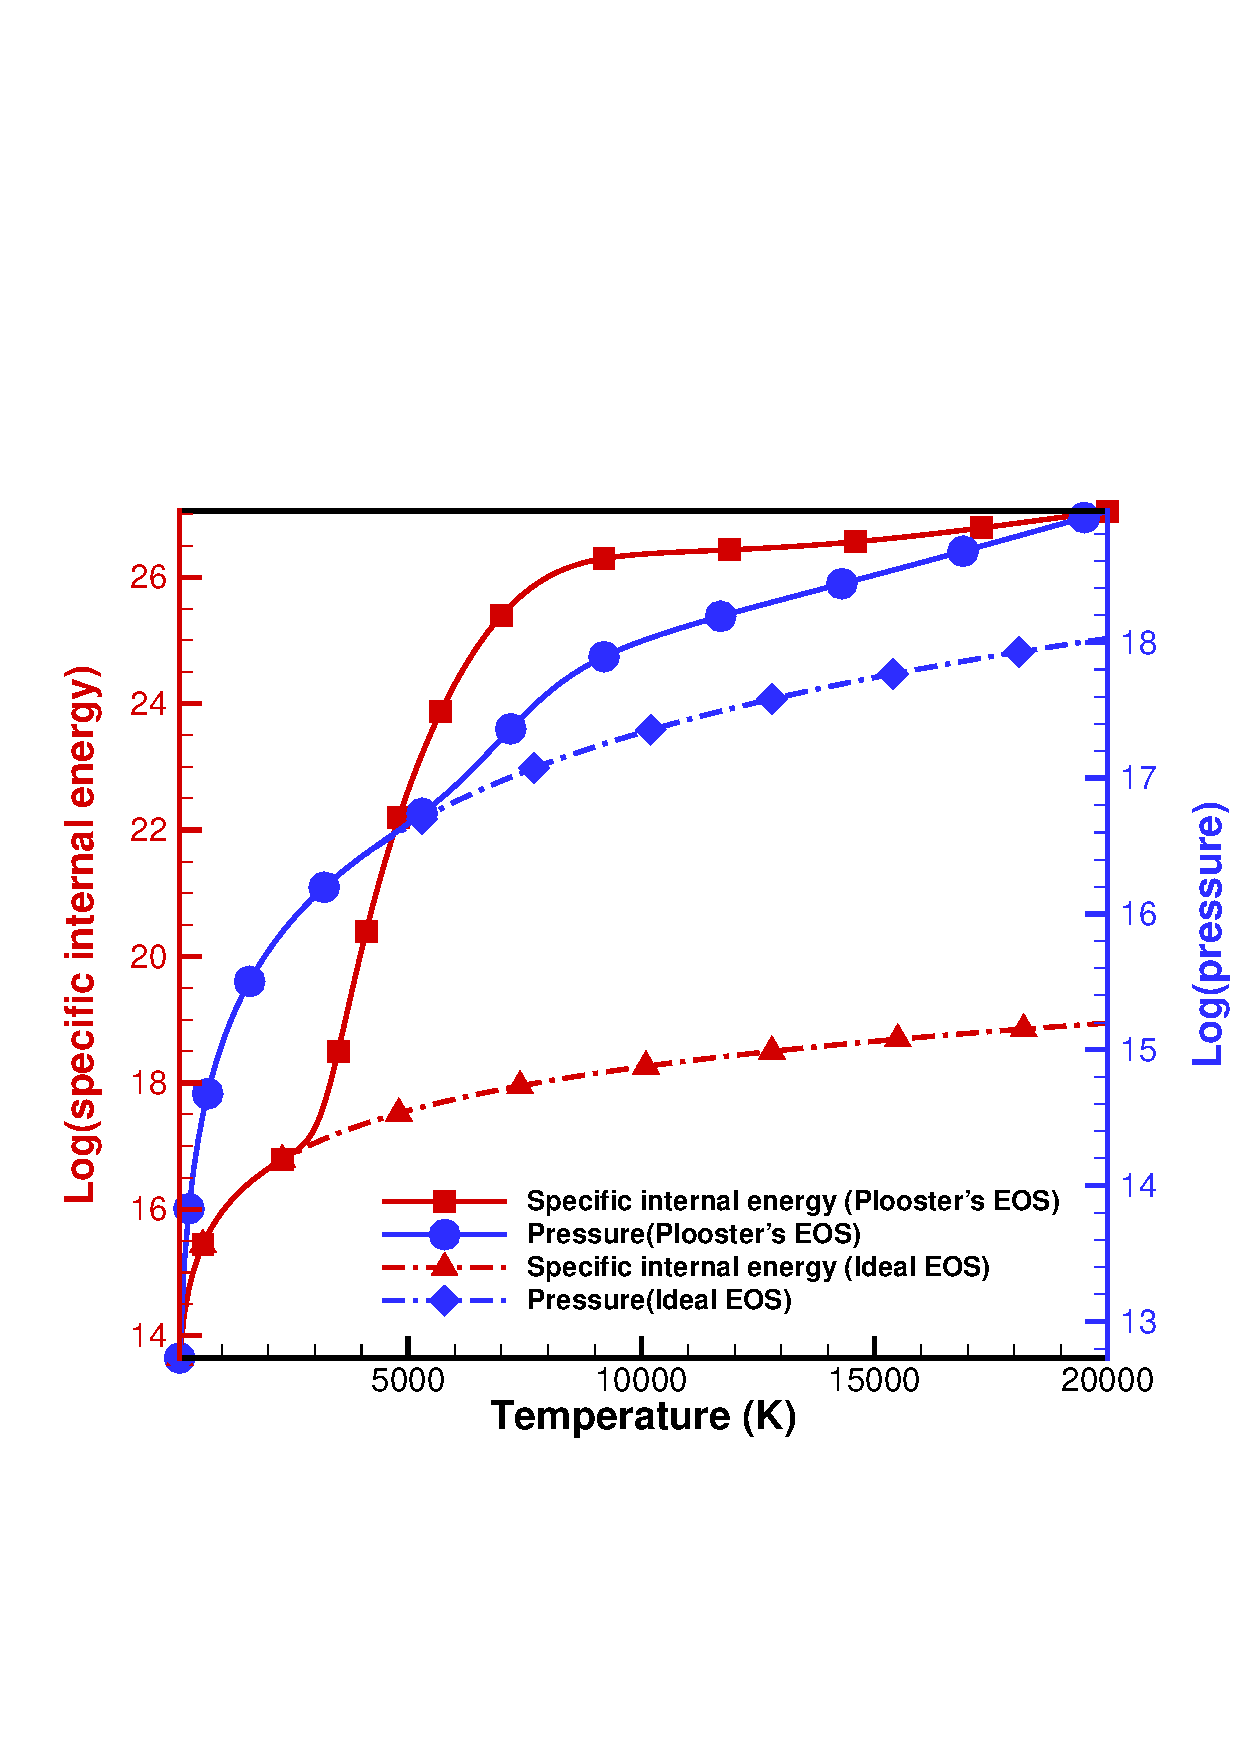
\includegraphics[width = 0.75\textwidth]{PIE}
    \caption{\textit{Variation of specific internal energy ($\epsilon$) and pressure ($p$) with temperature ($\theta$) for Plooster's EoS. At temperatures higher than 4,000 K, the internal energy and pressure deviates drstically from the ideal gas EoS due to high temperature effects such as dissociation and ionization. }}
    \label{fig:my_label}
\end{figure}
\end{document}
